% This is "sig-alternate.tex" V2.0 May 2012
% This is "sig-alternate.tex" V2.0 May 2012
% This file should be compiled with V2.5 of "sig-alternate.cls" May 2012
%
% This example file demonstrates the use of the 'sig-alternate.cls'
% V2.5 LaTeX2e document class file. It is for those submitting
% articles to ACM Conference Proceedings WHO DO NOT WISH TO
% STRICTLY ADHERE TO THE SIGS (PUBS-BOARD-ENDORSED) STYLE.
% The 'sig-alternate.cls' file will produce a similar-looking,
% albeit, 'tighter' paper resulting in, invariably, fewer pages.
%
% ----------------------------------------------------------------------------------------------------------------
% This .tex file (and associated .cls V2.5) produces:
%       1) The Permission Statement
%       2) The Conference (location) Info information
%       3) The Copyright Line with ACM data
%       4) NO page numbers
%
% as against the acm_proc_article-sp.cls file which
% DOES NOT produce 1) thru' 3) above.
%
% Using 'sig-alternate.cls' you have control, however, from within
% the source .tex file, over both the CopyrightYear
% (defaulted to 200X) and the ACM Copyright Data
% (defaulted to X-XXXXX-XX-X/XX/XX).
% e.g.
% \CopyrightYear{2007} will cause 2007 to appear in the copyright line.
% \crdata{0-12345-67-8/90/12} will cause 0-12345-67-8/90/12 to appear in the copyright line.
%
% ---------------------------------------------------------------------------------------------------------------
% This .tex source is an example which *does* use
% the .bib file (from which the .bbl file % is produced).
% REMEMBER HOWEVER: After having produced the .bbl file,
% and prior to final submission, you *NEED* to 'insert'
% your .bbl file into your source .tex file so as to provide
% ONE 'self-contained' source file.
%
% ================= IF YOU HAVE QUESTIONS =======================
% Questions regarding the SIGS styles, SIGS policies and
% procedures, Conferences etc. should be sent to
% Adrienne Griscti (griscti@acm.org)
%
% Technical questions _only_ to
% Gerald Murray (murray@hq.acm.org)
% ===============================================================
%
% For tracking purposes - this is V2.0 - May 2012

\documentclass{sig-alternate}

\usepackage{amsmath}
\usepackage{graphicx}
\usepackage{hyperref}
\usepackage{bbding}
\usepackage{pifont}
\usepackage{rotating}

\begin{document}
	%
	% --- Author Metadata here ---
	\conferenceinfo{WOODSTOCK}{'97 El Paso, Texas USA}
	%\CopyrightYear{2007} % Allows default copyright year (20XX) to be over-ridden - IF NEED BE.
	%\crdata{0-12345-67-8/90/01}  % Allows default copyright data (0-89791-88-6/97/05) to be over-ridden - IF NEED BE.
	% --- End of Author Metadata ---
	
	\title{Comparative Analysis of Multi Paradigms Languages}
	
	%
	% You need the command \numberofauthors to handle the 'placement
	% and alignment' of the authors beneath the title.
	%
	% For aesthetic reasons, we recommend 'three authors at a time'
	% i.e. three 'name/affiliation blocks' be placed beneath the title.
	%
	% NOTE: You are NOT restricted in how many 'rows' of
	% "name/affiliations" may appear. We just ask that you restrict
	% the number of 'columns' to three.
	%
	% Because of the available 'opening page real-estate'
	% we ask you to refrain from putting more than six authors
	% (two rows with three columns) beneath the article title.
	% More than six makes the first-page appear very cluttered indeed.
	%
	% Use the \alignauthor commands to handle the names
	% and affiliations for an 'aesthetic maximum' of six authors.
	% Add names, affiliations, addresses for
	% the seventh etc. author(s) as the argument for the
	% \additionalauthors command.
	% These 'additional authors' will be output/set for you
	% without further effort on your part as the last section in
	% the body of your article BEFORE References or any Appendices.
	
	\numberofauthors{8} %  in this sample file, there are a *total*
	% of EIGHT authors. SIX appear on the 'first-page' (for formatting
	% reasons) and the remaining two appear in the \additionalauthors section.
	%
	\author{
		% You can go ahead and credit any number of authors here,
		% e.g. one 'row of three' or two rows (consisting of one row of three
		% and a second row of one, two or three).
		%
		% The command \alignauthor (no curly braces needed) should
		% precede each author name, affiliation/snail-mail address and
		% e-mail address. Additionally, tag each line of
		% affiliation/address with \affaddr, and tag the
		% e-mail address with \email.
		%
		% 1st. author
		\alignauthor
		Shad Ahmed\\
		\affaddr{i14-1028}\\
		\affaddr{MS(CS)}
		% 2nd. author
		\alignauthor
		Faisal Mumtaz\\
		\affaddr{i16-1024}\\
		\affaddr{MS(CS)}
		% 3rd. author
		\alignauthor Umar Munir\\
		\affaddr{i16-1011}\\
		\affaddr{MS(CS)}
		\and  % use '\and' if you need 'another row' of author names
		% 4th. author
		% 4th. author
		\alignauthor Sharan Gohar \\
		\affaddr{i16-1064}\\
		\affaddr{MS(CS)}
		% 5th. author
		\alignauthor Mehreen Alam\\
		\affaddr{i16-1402}\\
		\affaddr{Phd(CS)}
		% 6th. author
		\alignauthor Shahid Hussain\\
		\affaddr{i17-1053}\\
		\affaddr{MS(CS)}
	}
	
	\maketitle
	\begin{abstract}
		Multiprogramming paradigms has gained immense popularity because of the wide spectrum of different paradigms covered. Not much work has been done to perform any comparative study and/or analysis of how various features are mapped onto different programming languages. This paper aims to highlights the concepts and usage of various features of different programming languages in multiprogramming languages. We have shortlisted our work to twelve programming languages Scala, Swift, Falcon, F\#, Rust, VB.net, C\#, Oz, Mozart, Matlab, R, and Python. On the other dimension, the features we have chosen to enhance our understanding of multiprogramming paradigm are Bound Checking, Type Safety, Exception Handling, Modularity, Compiled/Interpreted, Assertion, File Handling, Mutable, Immutable, Imperative Control and Explicit Concurrency. To the best of our knowledge, this is the first attempt to explore different features in depth and correlate them in their perspective of the above mentioned programming languages. The study revealed interesting patterns. While all languages support type safety, assertion, file-handling, exception handling, there is a variation in the behavior of the multi-paradigm programming languages when it comes to bound checking, meta-programming, compiled/interpreted, immutability, imperative control and explicit concurrency.
	\end{abstract}
	
	\keywords{theory of programming languages, multi-programming paradigms, features of programming languages}
	
	\section{Introduction}
	Programming paradigms are a way to classify programming languages based on their features. Languages can be classified into multiple paradigms. Some paradigms are concerned mainly with implications for the execution model of the language, such as allowing side effects, or whether the sequence of operations is defined by the execution model. Other paradigms are concerned mainly with the way that code is organized, such as grouping a code into units along with the state that is modified by the code. Yet others are concerned mainly with the style of syntax and grammar. Common programming paradigms include imperative, declarative and symbolic. The former allows side effects with object-oriented which groups code together with the state the code modifies and procedural which groups code into functions. Declarative which does not state the order in which operations execute with functional which disallows side effects and logic which has a particular style of execution model coupled to a particular style of syntax and grammar. The latter has a particular style of syntax and grammar as mentioned by \cite{kurt2012,Frans2012}.\\
For example, languages that fall into the imperative paradigm have two main features: they state the order in which operations occur, with constructs that explicitly control that order, and they allow side effects, in which state can be modified at one point in time, within one unit of code, and then later read at a different point in time inside a different unit of code. The communication between the units of code is not explicit. Meanwhile, in object-oriented programming, code is organized into objects that contain state that is only modified by the code that is part of the object. Most object-oriented languages are also imperative languages. In contrast, languages that fit the declarative paradigm do not state the order in which to execute operations. Instead, they supply a number of operations that are available in the system, along with the conditions under which each is allowed to execute. The implementation of the language's execution model tracks which operations are free to execute and chooses the order on its own. Pictorial representation of language to paradigm mapping is shown in the figure \ref{fig:langVSpara}.\\
\begin{figure}
  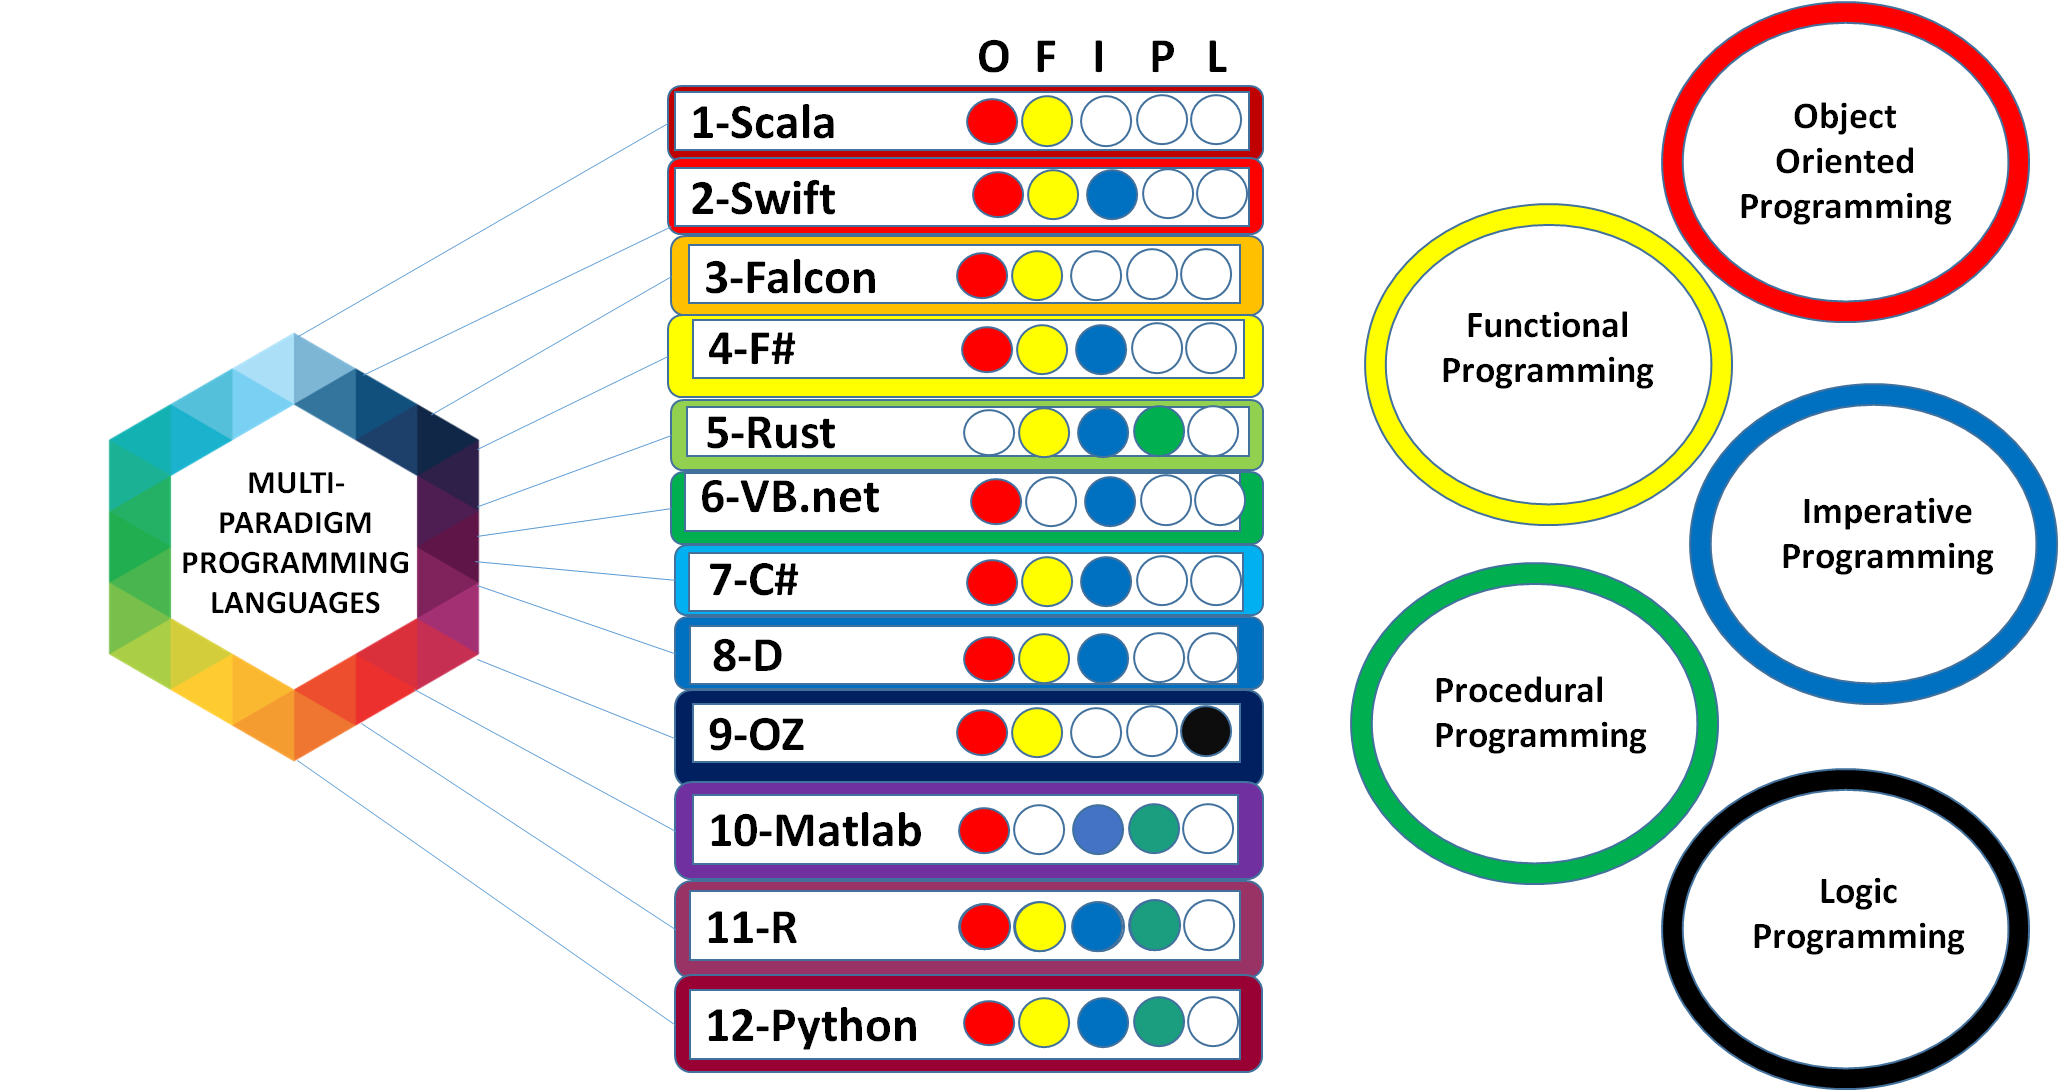
\includegraphics[width=\linewidth]{langVSparadigm.png}
  \caption{Programming Languages in perspective of Different Programming Paradigms}
	\label{fig:langVSpara}
\end{figure}

  Our work is a detailed study but not an exhaustive one. We have shortlisted the following multi-programming paradigm languages: Scala, Swift, Falcon, F\#, Rust, VB.net, C\#, Oz, Mozart, Matlab, R, and Python. Out of the comprehensive feature list we have focused our scope to the following only: Bound Checking, Type Safety, Exception Handling, Modularity, Compiled/Interpreted, Assertion, File Handling, Mutable, Immutable, Imperative Control and Explicit Concurrency. To the best of our knowledge, this is the first attempt to explore different features in depth and correlate them in their perspective of the above mentioned programming languages. The study revealed interesting patterns. While all languages support type safety, assertion, file-handling, exception handling, there is a variation in the behavior of the multi-paradigm programming languages when it comes to bound checking, meta-programming, compiled/interpreted, immutability, imperative control and explicit concurrency.\\
	The paper is organized as follows. Section I introduces the concept of multi-programming paradigm and its various features while section 2 explains the literature review. All the features are discussed in detail in section 3 followed by detailed discussion & analysis in section 4. We finally conclude in section 5 and mention the future work in section 6.\\
	
	\section{Related Work}
	Most Programming languages provide support for basic generic programming. Generic programming aims to express algorithms and data structures in a way to be broadly adaptable \cite{lr5}. Declarative programming languages provide more abstract level programming than imperative languages \cite{lr4}. They are characterized by their formal nature.  Modern programming languages are not just object-oriented but include multiple paradigms. Common programming paradigms are imperative, declarative and symbolic \cite{lr1}. Use of multiple programming paradigms help programmers in choosing suitable programming styles to get the job done \cite{lr2}. Existing work demonstrated that separate paradigms for solving problems is insufficient\cite{WinNT}. Hence analyzing multi-paradigm languages should be under study in order to manage work from multiple perspective. 
	
	\section{Features}
	
	\subsection{Bound Checking}
	In computer programming, bound checking is any method of whether variable detecting variable is within bound before it is used.  A failed bounds check usually results in the generation of some sort of exception signal.
	\subsubsection{Range checking}
	It is usually used to check that whether a number fits into a given type. A range check is a check to make sure a number is within a certain range; for example, range check will ensure that a value that will assign to a 16-bit integer is within the capacity of a 16-bit integer. Some range checks may be more restrictive; for example, a variable to hold the number of a calendar month may be declared to accept only the range 1 to 12.
	
	\subsubsection{Index checking}
	In index checking, a variable being used as an array index is within the bounds of the array. Index checking means all expressions indexing an array, the index value is checked against the bounds of the array, which were created when the array was defined, and if the index is out-of-bounds, an error occur and further execution is suspended. If a number outside of the upper range is used in an array, it may cause the program to crash, or may introduce security vulnerabilities, index checking is a part of many high-level languages.
	\begin{table}[]
		\centering
		\caption{Index Checking}
		\label{my-label}
		\begin{tabular}{|l|c|l|}
			\hline
			& Index checking                                              & Range checking                                                   \\ \hline
			Scala  &               \ding{52}                                              & \begin{tabular}[c]{@{}l@{}}\ding{52}\\   (statically check)\end{tabular} \\ \hline
			Swift  & \ding{52}                                                           & \ding{52}                                                                \\ \hline
			F\#    & \ding{52}                                                           & \ding{52}                                                                \\ \hline
			Rust   & \begin{tabular}[c]{@{}c@{}}\ding{52}\\   (at run time)\end{tabular} & -                                                                \\ \hline
			Vb.net & \ding{52}                                                           & \ding{52}                                                                \\ \hline
			C\#    & \ding{52}                                                           & \ding{52}                                                                \\ \hline
			D      & \ding{54}                                                           & \ding{52}                                                                \\ \hline
			Oz     & -                                                           & -                                                                \\ \hline
			Matlab & \ding{52}                                                           & \begin{tabular}[c]{@{}l@{}}\ding{52}(statically\\   check)\end{tabular}  \\ \hline
			Python & \ding{52}                                                           & \ding{52}                                                                \\ \hline
		\end{tabular}
	\end{table}
	
	\subsubsection{Examples}
	\subsubsection{Scala}
	Array representation in scala \\
	scala> val a1 = Array(1, 2, 3) \\
	Array[Int] = Array(1, 2, 3)
	
	\subsubsection{Swift}
	func contains(Bound)
	Returns a Boolean value indicating whether the given element is contained within the range.
	
	
	\subsection{Type Safety}
	The compiler will validate types and through an error if you assign a wrong type to a variable. 
	Type safety is checking for matched data types during compile time. For example, int a ="John" returns error as variable 'a' is an integer and we are assigning a string value. These data type mismatches are checked during compile time. Type safe code can access only the memory locations that it has permission to execute. Type safe code can never access any private members of an object. Type safe code ensures that objects are isolated from each other and are therefore safe for inadvertent or malicious corruption
	At compile time, we get an error when a type instance is being assigned to an incompatible type; hence preventing an error at run-time. So at compilation time itself, developers come to know such errors and code will be modified to correct the mistake. So developers get more confidence in their code. Run time type safety ensures, we don't get strange memory exceptions and inconsistent behavior in the application.
	
	\subsubsection{Scala}
	Scala is strongly type and smart about static type. Scala has powerful type inference. It will figure out itself mostly no need to tell it the types of your variables. 
	\subsubsection{Swift}
	Swift is type safe as it performs type checks when compiling code and flags any mismatched types as errors. This help in early catch and fix error in the development process. It provides type inference which basically means that coders do not require to spend more time in defining what types of variables they are using.
	\subsubsection{F\#}
	In F\#, static type checking can be used as an instant unit test, making sure that your code is correct at compile time. F\# is more type-safe than C\# since F\# compiler can catch errors that would only be detected at run-time in C\#.
	\subsubsection{Rust }
	Rust is a type-safe language. Rust has an escape valve from the safety rules when there is a need to use a raw pointer. This is called unsafe code, and while most Rust programs do not need it, how to use it and how it fits into Rust\'s overall safety scheme in \cite{WinNT}
	\\ https://www.safaribooksonline.com/library/view/programming-rust/9781491927274/ch21.html\#unsafe-code
	
	\subsubsection{VB.net}
	Type safety in .NET has been introduced to prevent the objects of one type from peeking into the memory assigned for the other object.
	\subsubsection{C\#}
	Type safety prevents assigning a type to another type when are not compatible.\\ \\
	public class Employee{}
	public class Student{}\\
	
	In the above example, Employee and Student are two incompatible types. We cannot assign an object of employee class to Student class variable. An error occurs during the compilation process if any such attempt is done. Type safety check happening at compile time are called static type checking
	Cannot implicitly convert type 'Program.Employee' to 'Program.Student'. \\ When tried to type cast object of wrong type. We get \\
	Unable to cast object of type 'first object' to 'second object'\\
	type checking happens at runtime, hence it is called runtime type checking\\
	\subsubsection{D}
	D has compile-time type safety. 
	\subsubsection{OZ }
	OZ also known as MOZART. Oz variables are single-assignment variables or more appropriately logic variables. A single assignment variable has a number of phases in its lifetime. Initially, it is introduced with unknown value while later it might be assigned a value and we say variable has become bound. Once a variable is bound, it cannot itself be changed.
	\subsubsection{Matlab}
	MATLAB is a loosely or weakly-typed language. Difference between MATLAB and a strongly-typed language is that there is no need to explicitly declare the types of the variables to use. For example, the declarations x=5; x='foo' immediately following one another are perfectly acceptable; the first declaration causes x to be treated as a number, the second changes its treatment to a string
	\subsubsection{Python}
	Python or Ruby are often referred to as dynamically typed languages, which throw exceptions to signal type errors occurring during execution

	% Please add the following required packages to your document preamble:
	% \usepackage[normalem]{ulem}
	% \useunder{\uline}{\ul}{}
	\begin{table}[]
		\centering
		\caption{Type Safety}
		\label{my-label}
		\begin{tabular}{|l|c|}
			\hline
			Languages & Type Safety                                                                                                                           \\ \hline
			Scala     & \begin{tabular}[c]{@{}c@{}}Strongly type, \\ Static type, \\ powerful type Inference\end{tabular}                                     \\ \hline
			Swift     & \begin{tabular}[c]{@{}c@{}}Type check at compile time, \\ Support type inference\end{tabular}                                         \\ \hline
			F\#       & \begin{tabular}[c]{@{}c@{}}Static Type Checking,\\ Compile Time\end{tabular}                                                          \\ \hline
			Rust      & \begin{tabular}[c]{@{}c@{}}Type Safe, \\ escape valve, \\ unsafe to use raw pointers\end{tabular}                                     \\ \hline
			VB.net    & Type safety use for memory security                                                                                                   \\ \hline
			C\#       & \begin{tabular}[c]{@{}c@{}}Static type checking,\\  type checking compile time\end{tabular}                                           \\ \hline
			D         & \begin{tabular}[c]{@{}c@{}}Type safe, \\ compile time\end{tabular}                                                                    \\ \hline
			Oz        & \begin{tabular}[c]{@{}c@{}}Single Assignment variables, \\ Once value is assigned to\\   variable it can never be change\end{tabular} \\ \hline
			Matlab    & \begin{tabular}[c]{@{}c@{}}Weakly type language, \\ no need to assign type explicitly,\end{tabular}                                   \\ \hline
			Python    & Dynamically type language,                                                                                                            \\ \hline
		\end{tabular}
	\end{table}
	
	\subsection{Exception Handling}
	An exception handler is a block of code that is executed if an exception occurs during the execution of some other block of code. In this sense, exceptions are a kind of control statement. Raising an exception transfers the flow-of-control to exception handling code. Users can also throw a self created exception.
	\begin{table}[]
		\centering
		\caption{Exception handling table}
		\begin{tabular}{|l|l|l|l|}
			\hline
			\begin{tabular}[c]{@{}l@{}}Lang\\ .\end{tabular}  & Throw                                                             & Handler                                                                                                                                                                                                              & Assertion                                                                                  \\ \hline
			\begin{tabular}[c]{@{}l@{}}Sca\\ la\end{tabular}  & throw                                                             & \begin{tabular}[c]{@{}l@{}}try \{ instructions \}\\  catch (exception) \\ \{ instructions\}\\  finally\{instructions\}\end{tabular}                                                                                  & \begin{tabular}[c]{@{}l@{}}Assert(stat\\ ement)\end{tabular}                               \\ \hline
			\begin{tabular}[c]{@{}l@{}}Swi\\ ft\end{tabular}  & \begin{tabular}[c]{@{}l@{}}throw exce\\ ption ()\end{tabular}     & \begin{tabular}[c]{@{}l@{}}do\\ \{ try expression ...\\  instructions \}\\  catch exception\\ \{ instructions \}\end{tabular}                                                                                        & \begin{tabular}[c]{@{}l@{}}assert(condi\\ tion,descrip\\ tion)\end{tabular}                \\ \hline
			\begin{tabular}[c]{@{}l@{}}Falc\\ on\end{tabular} & \begin{tabular}[c]{@{}l@{}}raise excep\\ tion\end{tabular}        & \begin{tabular}[c]{@{}l@{}}falcon.HTTPError\\ (status,title=None,\\ description=\\ None)\end{tabular}                                                                                                                &                                                                                            \\ \hline
			F\#                                               & \begin{tabular}[c]{@{}l@{}}raise exce\\ ption\end{tabular}        & \begin{tabular}[c]{@{}l@{}}try expression\\ with pattern \\ or\\ try expression \\ finally expression\end{tabular}                                                                                                   & \begin{tabular}[c]{@{}l@{}}assert cond\\ ition\end{tabular}                                \\ \hline
			Rust                                              & \begin{tabular}[c]{@{}l@{}}Err(excep\\ tion)\end{tabular}         & \begin{tabular}[c]{@{}l@{}}match fun\_nam(x,y)\\  \{\\           Ok(v) =\textgreater \{\\  println!("\{\}", v); \},\\           Err(err) =\textgreater \{\\   println!("\{\}", err);\\  \}\}\end{tabular}            &                                                                                            \\ \hline
			\begin{tabular}[c]{@{}l@{}}Vb\\ .Net\end{tabular} & \begin{tabular}[c]{@{}l@{}}throw excep\\ tion\end{tabular}        & \begin{tabular}[c]{@{}l@{}}Try\\ instructions\\ Catch exception \\ When condition\\   instructions\\   ...\\   Finally\\   instructions\\   End Try\end{tabular}                                                     & \begin{tabular}[c]{@{}l@{}}Debug.Ass\\ ert(condi\\ tion)\end{tabular}                      \\ \hline
			C\#                                               & \begin{tabular}[c]{@{}l@{}}throw excep\\ tion;\end{tabular}       & \begin{tabular}[c]{@{}l@{}}try \{ instructions \}\\ catch (exception) \\ \{ instructions\}\\ finally \{instructions\}\end{tabular}                                                                                   & \begin{tabular}[c]{@{}l@{}}Debug.Ass\\ ert(condi\\ tion);\end{tabular}                     \\ \hline
			D                                                 & throw                                                             & \begin{tabular}[c]{@{}l@{}}try \{ instructions \}\\ catch (exception) \\ \{ instructions\}\\ finally \{instructions\}\end{tabular}                                                                                   &                                                                                            \\ \hline
			Oz                                                & \begin{tabular}[c]{@{}l@{}}\{exception.\\ 'raise'X\}\end{tabular} & \begin{tabular}[c]{@{}l@{}}try S catch \\   Pattern\_1 then S1 \\   Pattern\_2 then S2 \\  finally \\    S\_final \\  end\end{tabular}                                                                               &                                                                                            \\ \hline
			
			R                                                 & throw()                                                           & \begin{tabular}[c]{@{}l@{}}tryCatch(\{\\       expr\},\\  war=function(w)\{\\  warning-handler-\\ code\},\\  error = function(e)\\  \{error-handler-\\ code\}, finally = \{\\       cleanup-code\\   \}\end{tabular} & \begin{tabular}[c]{@{}l@{}}assertError\\ (expr,verbo\\ se=FALSE)\end{tabular}              \\ \hline
			\begin{tabular}[c]{@{}l@{}}Pyth\\ on\end{tabular} & \begin{tabular}[c]{@{}l@{}}raise excep\\ tion\end{tabular}        & \begin{tabular}[c]{@{}l@{}}try:\\   Tab instructions\\   except exception:\\   Tab instructions\\   else:\\   Tab instructions\\   finally:\\   Tab  instruction\end{tabular}                                        & \begin{tabular}[c]{@{}l@{}}assert cond\\ ition\end{tabular}                                \\ \hline
		\end{tabular}
		
	\end{table}
	\subsection{Meta-programming}
	Meta-programming is the capability to adapt itself whereas meta stack overflow is the place to ask question about stack overflow itself. We can also say the ability to treat programs as their data. It means that a program can be designed to read, generate, analyze or transform other programs, and even modify itself while running. Meta-programming is not one specific technique, but rather an ensemble of concepts and techniques. There are two different ways of doing meta-programming: on the Syntax level and at Run-time as explained below.
	\begin{itemize}
		\item \textbf{Features for Syntax:} These are feature of languages through which Syntax meta-programming apply.
		\item \textbf{Features for Runtime:} These are feature of languages through which Run-time meta-programming apply.
	\end{itemize}
	\textbf{Reflection:} is the ability of a computer program to examine, introspect, and modify its own structure and behavior at runtime.
	\begin{table}[]
		\centering
		\caption{Meta Programming table}
		
		\begin{tabular}{|l|l|l|l|l|}
			\hline
			\begin{tabular}[c]{@{}l@{}}Prog. \\ Lang.\end{tabular} & \multicolumn{2}{l|}{Ways of Doing}                                                                          & \begin{tabular}[c]{@{}l@{}}Features\\ for compile\\ time\end{tabular} & \begin{tabular}[c]{@{}l@{}}Features\\ for Run\\ Time\end{tabular} \\ 
			
			\hline
			& \begin{tabular}[c]{@{}l@{}}Compile\\ Time\end{tabular} & \begin{tabular}[c]{@{}l@{}}Run\\ Time\end{tabular} &                                                                       &                                                                   \\ \hline
			R                                                      &                                                        & \Checkmark                                                  &                                                                       & Objects                                                           \\ \hline
			Scala                                                  & \Checkmark                                                      & \Checkmark                                                  & Reflection                                                            & Macros                                                            \\ \hline
			Swift                                                  & \Checkmark                                                      &                                                    &                                                                       & Templates                                                         \\ \hline
			Falcon                                                 & \Checkmark                                                      &                                                    &                                                                       & Macro                                                             \\ \hline
			F\#                                                    & \Checkmark                                                      & \Checkmark                                                  &                                                                       & Quotation                                                         \\ \hline
			Rust                                                   & \Checkmark                                                      &                                                    &                                                                       & Macros                                                            \\ \hline
			VB.net                                                 & \Checkmark                                                      & \Checkmark                                                  & Reflection                                                            & Reflection                                                        \\ \hline
			C\#                                                    &                                                        & \Checkmark                                                  &                                                                       & Objects                                                           \\ \hline
			D                                                      & \Checkmark                                                      &                                                    &                                                                       & Template                                                          \\ \hline
			Oz                                                     & x                                                      & x                                                  &                                                                       &                                                                   \\ \hline
			Matlab                                                 & x                                                      & x                                                  &                                                                       &                                                                   \\ \hline
			Python                                                 &                                                        & \Checkmark                                                  &                                                                       & \begin{tabular}[c]{@{}l@{}}meta-\\ classes\end{tabular}           \\ \hline
		\end{tabular}
		
	\end{table}
	
	\subsection{Compiled / interpreted}
	Compiled/interpreted: The difference lies not in the language but how the language has been implemented. A compiler translates the source code of the program into another language format that can be directly executed by a lower-level machine. This can be an abstract machine (such as .NET or the Java Virtual Machine) or the actual machine. In the latter case, the language format that is the target of the compiler is machine code. The translation from source code into lower-level code depends on the abstract syntax and on the operational semantics of the programming language. An interpreter executes the source code directly; informally, it may help to think of the interpreter as executing the program line by line. A more correct understanding is that the interpreter walks through the abstract syntax tree generated by the parser and executes each node in this tree. If a node is a leaf, the leaf is executed. If a node is an internal node, each sub-tree is visited and executed. Exactly how this is to be done depends on the abstract syntax and on the underlying semantics of the programming language.
	Out of the many programming languages in this world, some of them are called compiled languages while some are interpreted. For compilation, the software uses is called compiler while for interpreter is used for interpreted language. For a compiled language, an interpreter can be built but the reverse is impossible. That is, all the interpreted languages cannot be a compiled language. Additionally, being interpreted or compiled is not the property of the programming languages, but the design of some languages make them unsuitable for native code generation. Figure \ref{fig:compiledInterpreted} gives the complete picture.\\
\begin{figure}
  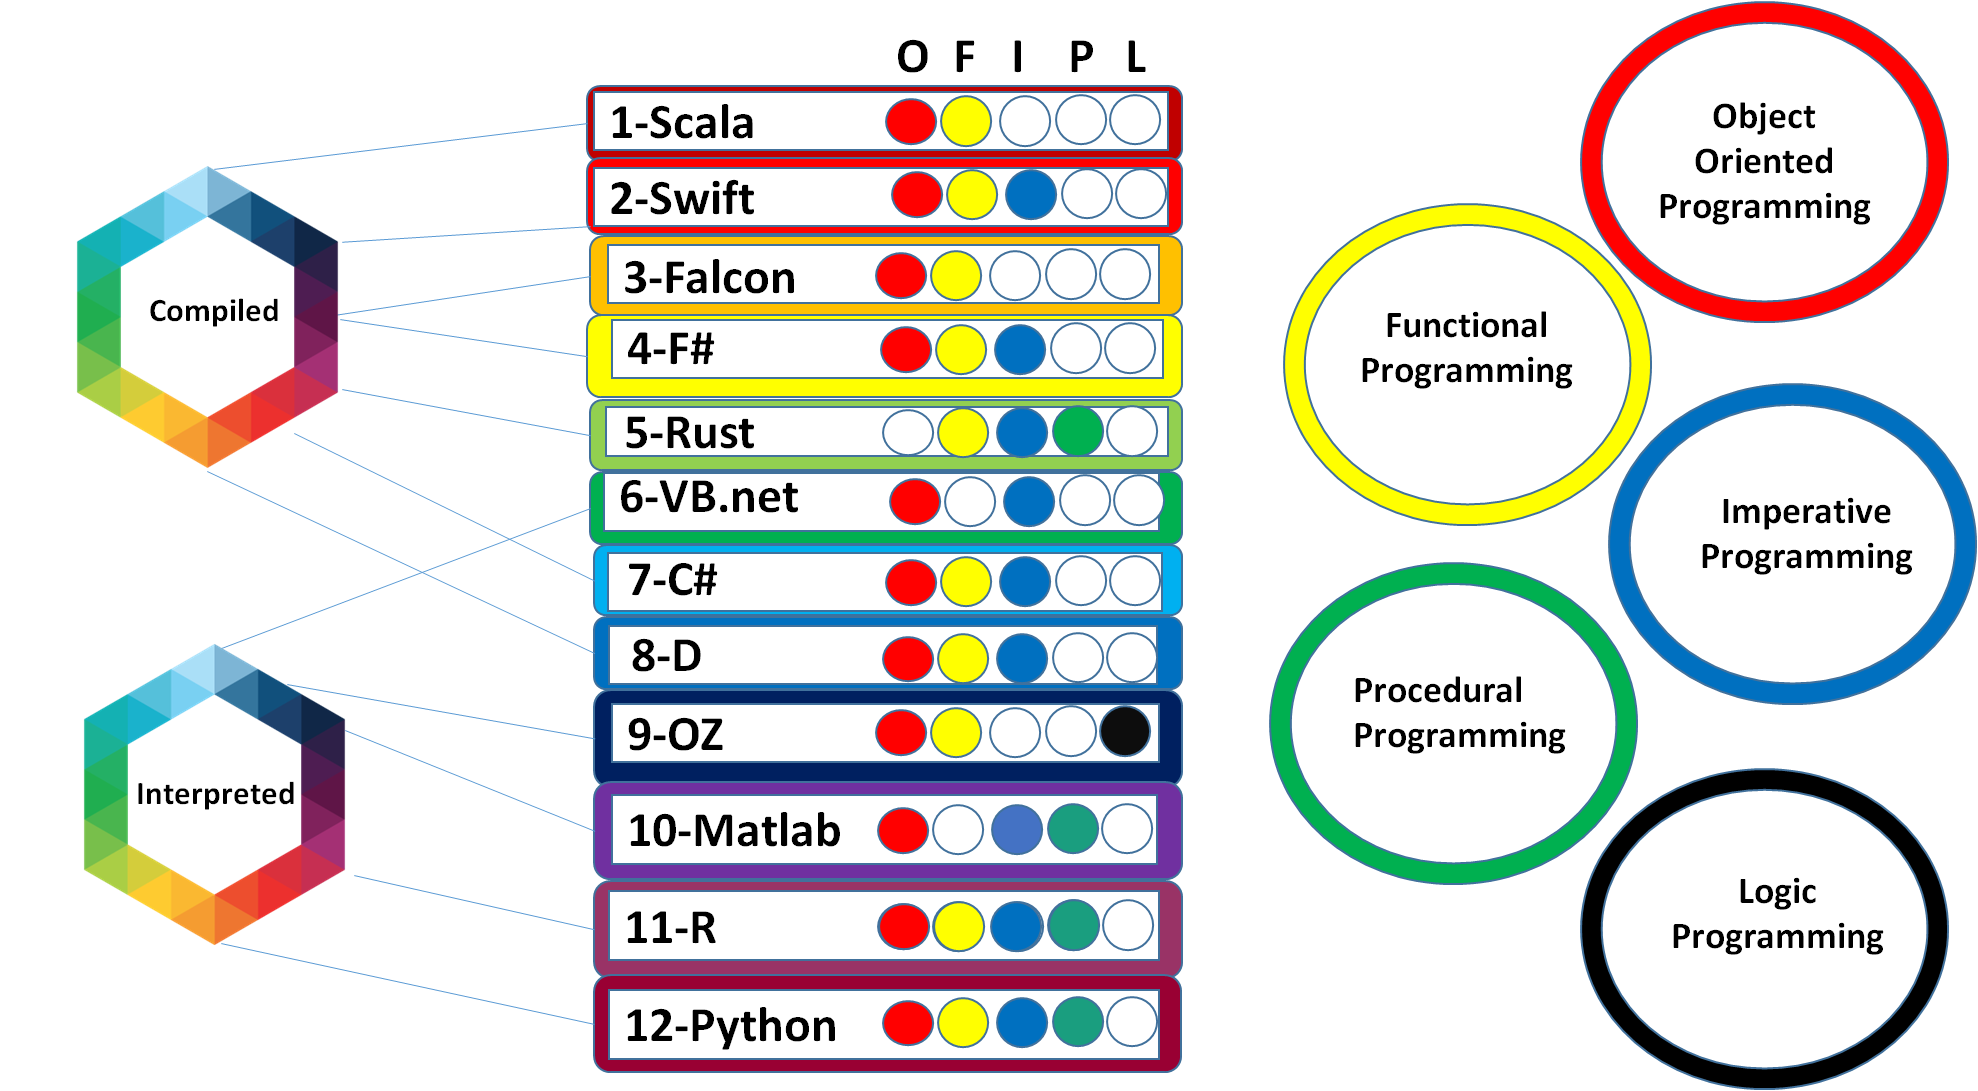
\includegraphics[width=\linewidth]{compiledInterpreted.png}
  \caption{Pictorial Representation of Programming Languages in perspective of Compiled and Interpreted Languages}
	\label{fig:compiledInterpreted}
\end{figure}

	\begin{table*}[]
		\centering
		\caption{Compiled/interpreted]}
		\label{my-label}
		\begin{tabular}{|l|l|l|}
			\hline
			\textbf{}        & \textbf{compiled}                                                                                                                                                                                                                                                                                                                                              & \textbf{interpreted}                                                                                                              \\ \hline
			\textbf{Scala}   & \begin{tabular}[c]{@{}l@{}}actually a compiled , wherein\\   everything you type gets compiled \\  to the byte code and it runs within\\  the  JVM.\end{tabular}                                                                                                                                                                                               & illusion of interpreted                                                                                                           \\ \hline
			\textbf{Swift}   & compiled                                                                                                                                                                                                                                                                                                                                                       &                                                                                                                                   \\ \hline
			\textbf{Falcon}  & \begin{tabular}[c]{@{}l@{}}compiled, The Falcon compiler \\ contains a meta-compiler{[}23{]} that\\   supports macro expansions. A \\ Falcon Virtual Machine in the \\  standard compiler drives the \\  meta-compiler. Output generated\\  from the meta-compiler is sent to\\   the language lexer as if part of\\  the original source.\end{tabular}        &                                                                                                                                   \\ \hline
			\textbf{F\#}     & \begin{tabular}[c]{@{}l@{}}compiled, open source cross platform \\ compiler from F\# Software  Foundation\end{tabular}                                                                                                                                                                                                                                         &                                                                                                                                   \\ \hline
			\textbf{Rust}    & \begin{tabular}[c]{@{}l@{}}compiled.\\   First, the Rust compiler does all the\\  Rust specific stuff like type and \\ borrow checking; in the end, it \\ generates LLVM-IR. IR stands \\ for intermediate representation \\ and it's comparable to assembly,\\  but a tiny bit more high level and\\  most importantly: \\ platform independent.\end{tabular} &                                                                                                                                   \\ \hline
			\textbf{Vb .Net} & \begin{tabular}[c]{@{}l@{}}version 6 and above, \\ both compiled and interpreted\end{tabular}                                                                                                                                                                                                                                                                  & interpreted                                                                                                                       \\ \hline
			\textbf{C\#}     & compiled                                                                                                                                                                                                                                                                                                                                                       &                                                                                                                                   \\ \hline
			\textbf{D}       & compiled                                                                                                                                                                                                                                                                                                                                                       &                                                                                                                                   \\ \hline
			\textbf{Oz}      & \begin{tabular}[c]{@{}l@{}}ding{52}, Oz code can be\\   compiled into command line\\  executables. The compiled \\ code is not native binary, \\ but a shell script-wrapper\\  with embedded Oz virtual\\  machine bytecode.\end{tabular}                                                                                                                           &                                                                                                                                \\ \hline
			\textbf{Matlab}  &                                                                                                                                                                                                                                                                                                                                                                & \begin{tabular}[c]{@{}l@{}},  you can\\   write code and just \\ execute it from the IDE,\\  without compilation.\end{tabular} \\ \hline
			\textbf{R}       & \begin{tabular}[c]{@{}l@{}}an interface to compiled code,\\   because all key routines are run \\  in compiled code (through .C, \\ .Call., .Internal, .Primitive interfaces,\\  etc.) But does not compile\end{tabular}                                                                                                                                       & \ding{52}                                                                                                                               \\ \hline
			\textbf{Python}  &                                                                                                                                                                                                                                                                                                                                                                & \ding{52}                                                                                                                               \\ \hline
		\end{tabular}
\end{table*}
	
	
	\subsection{Assertion}
	Assertion: specifies that a program satisfies certain conditions at particular points in its execution. An assertion violation indicates a bug in the program. Thus, assertions are an effective means of improving the reliability of programs and function as a systematic debugging tool. There are three types of assertion: pre-conditions, post-conditions and invariants. Preconditions specify conditions at the start of a function; post-conditions specify conditions at the end of a function while invariants specify conditions over a defined region of a program. Asserts are to be used primarily for checking parameter types, classes, or values, checking data structure invariants, checking "can't happen" situations (duplicates in a list, contradictory state variables) or after calling a function, to make sure that its return is reasonable. However, asserts are not to be used for handling run-time errors, like entering a negative number when positive is needed. But used to catching the program errors. Figure \ref{fig:assert} gives the complete picture.\\
\begin{figure}
  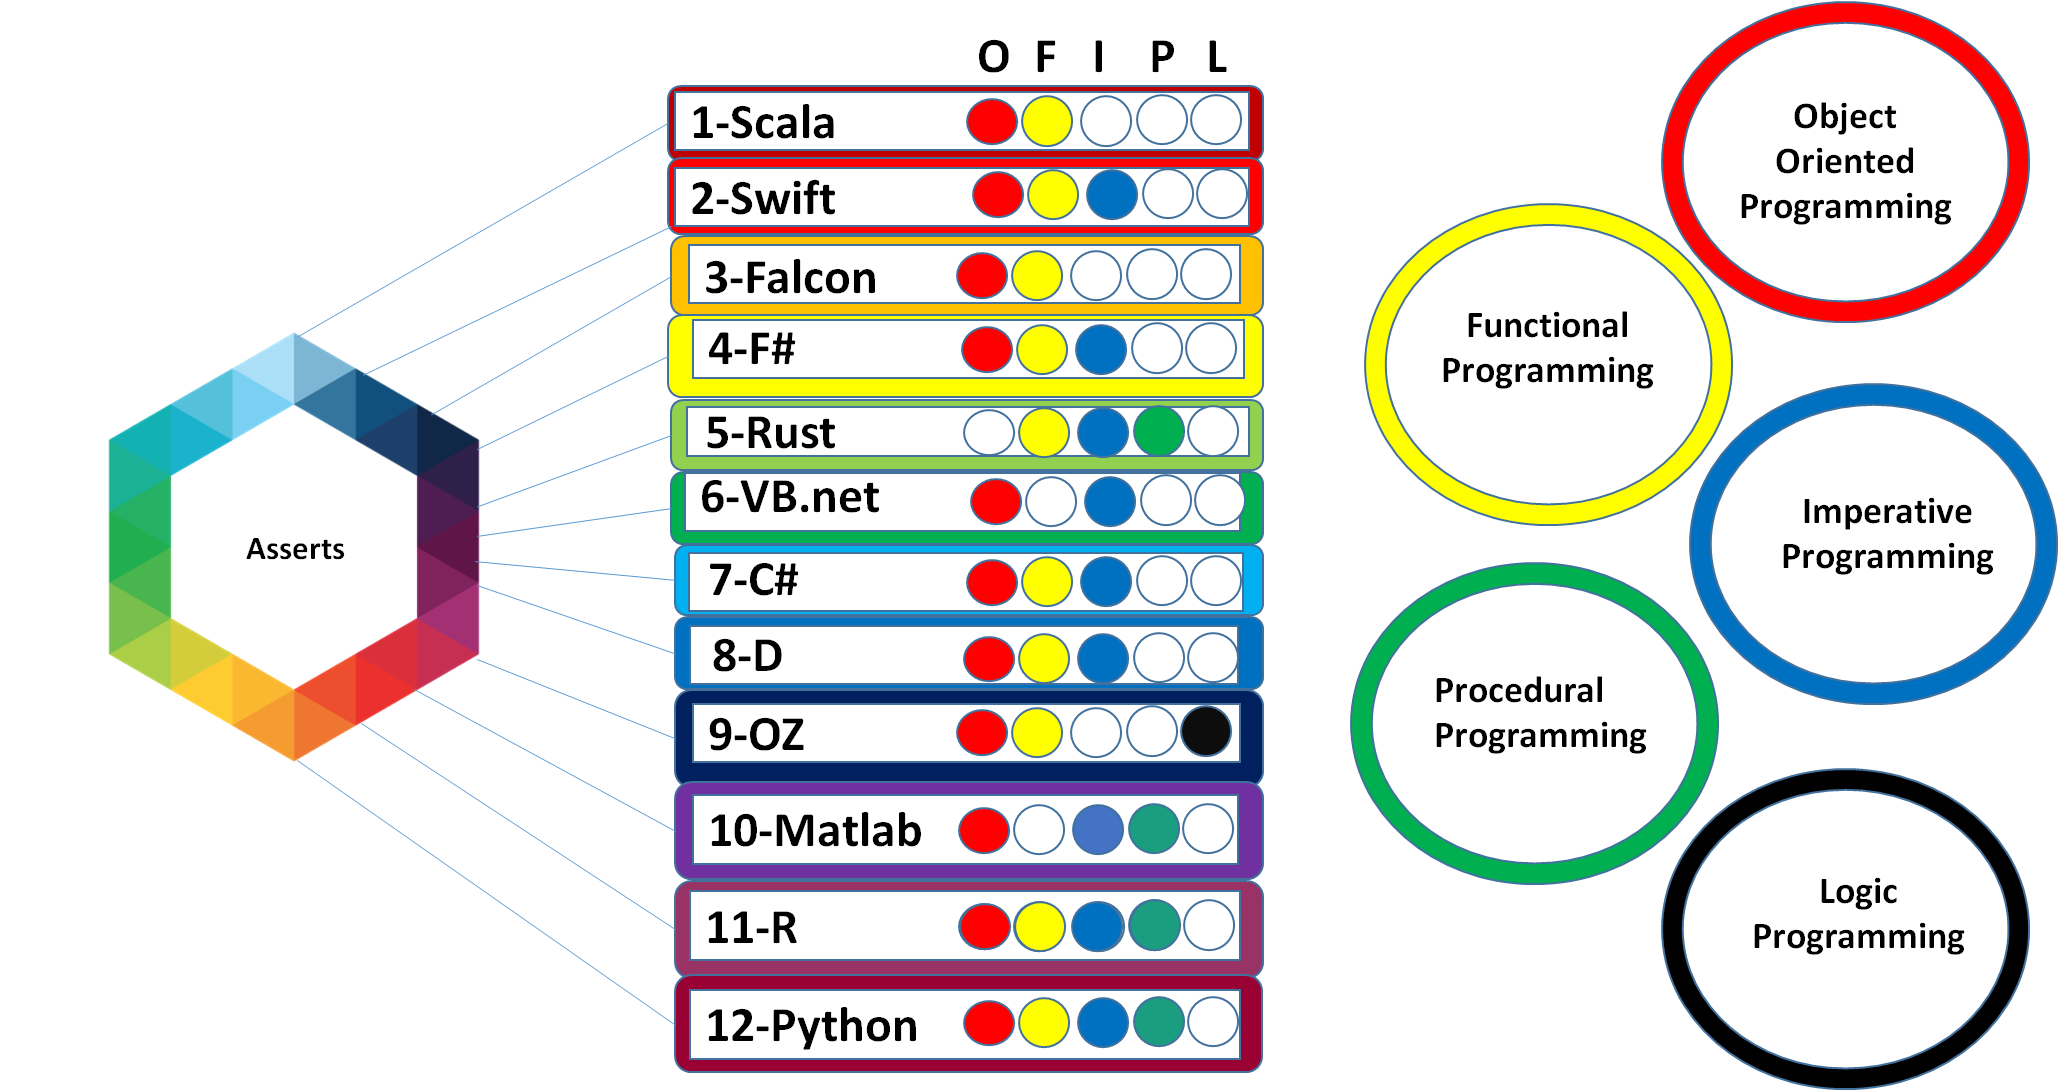
\includegraphics[width=\linewidth]{assert.png}
  \caption{Pictorial Representation of Programming Languages in perspective of Assertion}
	\label{fig:assert}
\end{figure}

	\begin{table*}[]
		\centering
	\caption{Assertion - 1}
	\label{my-label}
	\begin{tabular}{|l|l|l|l|l|l|}
		\hline
		\textbf{}        & \textbf{\begin{tabular}[c]{@{}l@{}}Pre-Post \\ conditions\end{tabular}} & \textbf{Quantification} & \textbf{\begin{tabular}[c]{@{}l@{}}Pre-State \\ Values\end{tabular}} & \textbf{\begin{tabular}[c]{@{}l@{}}Global \\ Assertions\end{tabular}} & \textbf{\begin{tabular}[c]{@{}l@{}}Language \\ Integration\end{tabular}}                                                                                                                                                                                               \\ \hline
		\textbf{Scala}   & ding{54}                                                                      &                         & \ding{54}                                                                  & \ding{54}                                                                   & import org.scalatest.Assertions.\_                                                                                                                                                                                                                                     \\ \hline
		\textbf{Swift}   &                                                                         &                         &                                                                      &                                                                       &                                                                                                                                                                                                                                                                        \\ \hline
		\textbf{Falcon}  & \ding{52}                                                                     & \ding{52}                     & \ding{54}                                                                  & \ding{52}                                                                   & import falcon                                                                                                                                                                                                                                                          \\ \hline
		\textbf{F\#}     & \ding{54}                                                                     & \ding{54}                     & \ding{54}                                                                  & \ding{54}                                                                   & \begin{tabular}[c]{@{}l@{}}open FsUnit\\   {[}\textless{}AbstractClass\textgreater{}{]}{[}\textless{}Sealed\textgreater{}{]}type Assert = class end\end{tabular}                                                                                                       \\ \hline
		\textbf{Rust}    & \ding{52}                                                                     & \ding{52}                     & \ding{52}                                                                  & \ding{52}                                                                   &                                                                                                                                                                                                                                                                        \\ \hline
		\textbf{Vb .Net} & \ding{54}                                                                     & \ding{54}                     & \ding{54}                                                                  & \ding{54}                                                                   & \begin{tabular}[c]{@{}l@{}}Debug.Assert Method\\   System.Diagnostics\\   Namespace\\   Public NotInheritable Class Assert\end{tabular}                                                                                                                                \\ \hline
		\textbf{C\#}     & \ding{54}                                                                     & \ding{54}                     & \ding{54}                                                                  & \ding{54}                                                                   & \begin{tabular}[c]{@{}l@{}}assert method in class Debug\\   public static class Assert\end{tabular}                                                                                                                                                                    \\ \hline
		\textbf{D}       & \ding{54}                                                                     & \ding{54}                     & \ding{54}                                                                  & \ding{54}                                                                   & \ding{54}                                                                                                                                                                                                                                                                    \\ \hline
		\textbf{Oz}      & \ding{52}                                                                     & \ding{52}                     & \ding{52}                                                                  & \ding{52}                                                                   & export Literals Assert                                                                                                                                                                                                                                                 \\ \hline
		\textbf{Matlab}  & \ding{52}                                                                     & \ding{52}                     & \ding{52}                                                                  & \ding{54}                                                                   & \ding{52}, python, c,c++, C\#, java, fortran                                                                                                                                                                                                                                 \\ \hline
		\textbf{R}       & \ding{52}                                                                     & \ding{52}                     & \ding{52}                                                                  & \ding{52}                                                                   & \begin{tabular}[c]{@{}l@{}}assertthat\\   -assert\_that() signal an error\\   -see\_if() returns\\   a logical value, with the error message as an attribute.\\   -validate\_that() returns TRUE on\\   success, otherwise returns the error as a string.\end{tabular} \\ \hline
		\textbf{Python}  & \ding{52}                                                                     & \ding{52}                     & \ding{54}                                                                  & \ding{54}                                                                   & assert method                                                                                                                                                                                                                                                          \\ \hline
		\textbf{}        & \begin{tabular}[c]{@{}l@{}}Pre-Post \\ conditions\end{tabular}          & Quantification          & \begin{tabular}[c]{@{}l@{}}Pre-State \\ Values\end{tabular}          & \begin{tabular}[c]{@{}l@{}}Global \\ Assertions\end{tabular}          & \begin{tabular}[c]{@{}l@{}}Language \\ Integration\end{tabular}                                                                                                                                                                                                        \\ \hline
	\end{tabular}
\end{table*}



\begin{table*}[]
\centering
\caption{Assertion - 2}
\label{my-label}
\begin{tabular}{|l|l|l|l|l|}
	\hline
	\textbf{}        & \textbf{Security Levels}                                                      & \textbf{\begin{tabular}[c]{@{}l@{}}enabling \\ / disabling \\ assertions\end{tabular}}                                                                                                  & \textbf{\begin{tabular}[c]{@{}l@{}}debugging\\  support\end{tabular}}                          & \textbf{inheritance}                                                                                                               \\ \hline
	\textbf{Scala}   & \ding{54}                                                                           & \begin{tabular}[c]{@{}l@{}}assume\\   fail\\   cancel\\   succeed\\   intercept\\   exception\\   assertDoesNotCompile\\   assertCompiles\\   assertTypeError\\   withClue\end{tabular} & \begin{tabular}[c]{@{}l@{}}Scala Debugger\\    Intellij IDEA\end{tabular}                      & \begin{tabular}[c]{@{}l@{}}subclass inherits any \\ non-overridden methods \\ in super class that \\ contains asserts\end{tabular} \\ \hline
	\textbf{Swift}   &                                                                               &                                                                                                                                                                                         &                                                                                                &                                                                                                                                    \\ \hline
	\textbf{Falcon}  & \ding{54}                                                                           & \ding{54}                                                                                                                                                                                     & \begin{tabular}[c]{@{}l@{}}falcon command \\ line interpreter\end{tabular}                     & \ding{54}                                                                                                                                \\ \hline
	\textbf{F\#}     & \ding{54}                                                                           & \ding{54}                                                                                                                                                                                     & \begin{tabular}[c]{@{}l@{}}.NET debugger\\   System. Diagnostic.\\  Debug. Assert\end{tabular} & \begin{tabular}[c]{@{}l@{}}subclass inherits any \\ non-overridden methods \\ in super class that \\ contains asserts\end{tabular} \\ \hline
	\textbf{Rust}    & \ding{54}                                                                           & \ding{52}                                                                                                                                                                                     & \begin{tabular}[c]{@{}l@{}}debug\_assert!\\   interpreter\end{tabular}                         & \ding{54}                                                                                                                                \\ \hline
	\textbf{Vb .Net} & \ding{54}                                                                           & \ding{54}                                                                                                                                                                                     & \begin{tabular}[c]{@{}l@{}}VBasic .Net \\ Debugger\end{tabular}                                & \ding{52}                                                                                                                                \\ \hline
	\textbf{C\#}     & \ding{54}                                                                           & \begin{tabular}[c]{@{}l@{}}conditional compilation\\   C\# - .NET�s Base \\ Class Library (BCL) \\ supports similar facility\\   for C\#, C++ and VBA.\end{tabular}                     & C\# debugger                                                                                   & \begin{tabular}[c]{@{}l@{}}subclass inherits any \\ non-overridden methods \\ in super class that \\ contains asserts\end{tabular} \\ \hline
	\textbf{D}       & \ding{54}                                                                           & \ding{54}                                                                                                                                                                                     & \ding{54}                                                                                            & \ding{54}                                                                                                                                \\ \hline
	\textbf{Oz}      & \ding{54}                                                                           & \ding{54}                                                                                                                                                                                     & \ding{54}                                                                                            & \ding{54}                                                                                                                                \\ \hline
	\textbf{Matlab}  & \begin{tabular}[c]{@{}l@{}}fatalAssertThat\\   fataAssertWarning\end{tabular} & \begin{tabular}[c]{@{}l@{}}\ding{52}\\   global NDEBUG;\\  NDEBUG=true;\end{tabular}                                                                                                          & \begin{tabular}[c]{@{}l@{}}\ding{52}\\   matlab\end{tabular}                                         & \ding{54}                                                                                                                                \\ \hline
	\textbf{R}       & \ding{54}                                                                           & \begin{tabular}[c]{@{}l@{}}\ding{52}\\   customized assert \\ statements \\ can also be written\end{tabular}                                                                                  & \ding{54}                                                                                            & \ding{54}                                                                                                                                \\ \hline
	\textbf{Python}  & \ding{54}                                                                           & \ding{52}                                                                                                                                                                                     & \begin{tabular}[c]{@{}l@{}}\ding{52}\\   python interpreter\end{tabular}                             & \ding{52}                                                                                                                                \\ \hline
	\textbf{}        & Security Levels                                                               & \begin{tabular}[c]{@{}l@{}}enabling \\ / disabling \\ assertions\end{tabular}                                                                                                           & \begin{tabular}[c]{@{}l@{}}debugging \\ support\end{tabular}                                   & inheritance                                                                                                                        \\ \hline
\end{tabular}
	\end{table*}
	\subsection{Conditional compilation}
	Conditional compilation is a method of producing different results by different parameters provided during compilation of the program. This technique is used when a program is built for different platforms or to run or not to run specific portion of code in a certain condition or to run a program with different version etc. For example, in case of error program should display a debug report so, in C, \#ifdef will be used to define a debug. In HTML, different display sizes can be defined for different platforms like desktop, tablet, mobile etc. A compiler may be set to define different operating systems like windows, linux, mac etc. to compile the code accordingly or for javaascript versioning for different browsers. 
	
	\begin{table}[]
		\centering
		\caption{Table of conditional compilation}
		\label{my-label}
		\begin{tabular}{|l|l|}
			\hline
			& Conditional Compilation                                                                                                                                      \\ \hline
			Scala   & \begin{tabular}[c]{@{}l@{}}scala.language.experimental.macros\\ elidable\end{tabular}                                                                        \\ \hline
			Swift   & \#if condition                                                                                                                                               \\ \hline
			Falcon  &                                                                                                                                                              \\ \hline
			F\#     &                                                                                                                                                              \\ \hline
			Rust    & \begin{tabular}[c]{@{}l@{}}\#\{{[}\}cfg\{{]}\}\\ for example \#\{{[}\}cfg(foo)\{{]}\}\end{tabular}                                                           \\ \hline
			Vb .net & \#if?then?\#else                                                                                                                                             \\ \hline
			C\#     & \#if                                                                                                                                                         \\ \hline
			D       & \begin{tabular}[c]{@{}l@{}}debug \{    // ... conditionally \\ compiled code ... \} else \{    // ... code \\ that is compiled otherwise ... \}\end{tabular} \\ \hline
			Oz      &                                                                                                                                                              \\ \hline
			Matlab  & \begin{tabular}[c]{@{}l@{}}\#if (condition) \{do something\} \\ \#else \{do something else\} \#end\end{tabular}                                              \\ \hline
			R       &                                                                                                                                                              \\ \hline
			Python  &                                                                                                                                                              \\ \hline
		\end{tabular}
	\end{table}
	
	\subsection{File handling}
	File handling is used where data is required to be provided to the program from and to an external source, not using keyboard during program compilation. Data is stored in files that will be used by program during execution. Using file handling technique, data will be read from the file as soon as it requires without waiting for human user to input. Similarly information (output) will be saved to file and program execution will proceed without user to make any interaction like "Press any key to continue...". File handling has three steps 1) Opening a file: Opening a file for reading data from or writing data to an external file. 2) Reading/writing data: Reading data as input for program to store values in variables and operate on it or writing output to the file. 3) Closing a file: Closing the file once it's use is over. A file can be closed as soon as it's use is over or it can be closed at the end of program execution before closing the program.
	\begin{table}[]
\centering
\caption{Table of File Handling}
\label{my-label}
\begin{tabular}{|l|l|}
\hline
Languages & File Handling                                                                                                                                                                                                                                                                                        \\ \hline
Scala     & \begin{tabular}[c]{@{}l@{}}import scala.io.Source,\\ Source.fromFile("any  file")\end{tabular}                                                                                                                                                                                                       \\ \hline
Swift     & Yes                                                                                                                                                                                                                                                                                                  \\ \hline
Falcon    & Yes                                                                                                                                                                                                                                                                                                  \\ \hline
F\#       & open System.IO                                                                                                                                                                                                                                                                                       \\ \hline
Rust      & io::Result\textless{}T\textgreater{}                                                                                                                                                                                                                                                                 \\ \hline
Vb .net   & \begin{tabular}[c]{@{}l@{}}Imports System.IO, FileStream =\\ New FileStream( "sample.txt", \\ FileMode.OpenOrCreate,\\ FileAccess.ReadWrite)\end{tabular}                                                                                                                                            \\ \hline
C\#       & \begin{tabular}[c]{@{}l@{}}FileStream \textless{}object\_name\textgreater = new\\ FileStream( \textless{}file\_name\textgreater{}, \\ \textless{}FileMode Enumerator\textgreater{},\\ \textless{}FileAccess Enumerator\textgreater{},\\ \textless{}FileShare Enumerator\textgreater{});\end{tabular} \\ \hline
D         & \begin{tabular}[c]{@{}l@{}}import std.file;\\ File file = File("test.txt", "w");\\ file.writeln("hello");\\ string s = file.readln();\end{tabular}                                                                                                                                                   \\ \hline
Oz        & Yes                                                                                                                                                                                                                                                                                                  \\ \hline
Matlab    & \begin{tabular}[c]{@{}l@{}}A = fscanf(fileID,formatSpec),\\ {[}A,count{]} = fscanf(\_\_\_)\\ A = fscanf(fileID,formatSpec,\\ sizeA)\end{tabular}                                                                                                                                                     \\ \hline
R         & \begin{tabular}[c]{@{}l@{}}list.files(file.path("F:", "git", \\ "roxygen2")) file.create,\\ file.exists, file.remove, file.rename,\\ file.append, file.copy, file.symlink,\\ file.link(from, to)\end{tabular}                                                                                        \\ \hline
Python    & file\_object  = open(?filename?, ?mode?)                                                                                                                                                                                                                                                             \\ \hline
\end{tabular}
\end{table}
	\subsection{Immutable}
	In muti-paradigm programming languages, an immutable object is an object whose state cannot be modified after it is created. This is in contrast to a mutable object (changeable object), which can be modified after it is created. In some cases, an object is considered immutable even if some internally used attributes change but the object's state appears to be unchanging from an external point of view. For example, an object that uses memorization to cache the results of expensive computations could still be considered an immutable object.
	
	

	\subsection{Mutable}
	A mutable object, in contrast to immutable, has data fields that can be altered. One or more of its methods will change the contents of the object, or has a property that, when written into, will change the value of the object.
	If you have a mutable object- the most similar one to String is StringBuffer inC\#- then you have to make a copy of it if you want to be absolutely sure it would not change out from under you. This is why mutable objects are dangerous to use as keys in any form of Dictionary or Set- the objects themselves could change, and the data structure would have no way of knowing, leading to corrupt data that would, eventually, crashing the program. However, the contents can be changed with much more memory efficiency than making a complete copy. Generally, the right thing to do is use mutable objects while creating something, and immutable objects once creation is done. This applies to objects that have immutable forms, of course; most of the collections don't. It's often useful to provide read-only forms of collections, though, which is the equivalent of immutable, when sending the internal state of collection to other contexts- otherwise, something could take that return value. This could do something to to it, e.g corrupt it. 
	
	\begin{table}[]
		\centering
		\caption{Mutable programming features in different languages}
		\label{my-label}
		\begin{tabular}{|l|l|}
			\hline
			\multicolumn{2}{|c|}{Mutable}                     \\ \hline
			Scala  & var maxValue = 100                         \\ \hline
			Swift  & var (firstNumber, secondNumber) = (10, 42) \\ \hline
			Falcon & array={[}1,2,3{]}                          \\ \hline
			F\#    & let a = 1                                  \\ \hline
			Rust   & let a = 1                                  \\ \hline
			Vb.net & Dim num1  as Integer = 1                   \\ \hline
			C\#    & float PI = 3.14149                         \\ \hline
			D      & mutable int len = 1                        \\ \hline
			Oz     & \{Browse \{4+2\} div 2\}                   \\ \hline
			Matlab & h = 6.626068e-34;                          \\ \hline
			R      & a\textless{}- 1                            \\ \hline
			Python & var a = 1                                  \\ \hline
		\end{tabular}
	\end{table}
	
	\subsection{Imperative Control}
	
	Imperative control in programming languages allow to explicitly define the execution order of program statements and expressions. Method or procedure is a sequence of control constructs. A method could be invoked, with or without passing parameters and its result could be returned to the caller. Body of method/procedure may contain imperative control expressions like if�else, switch statements and iteration statements like for, while, do etc.
	\newline
	In the true spirit of knowledge sharing, aiming to be practical, informative, and digestible, so much so that the reader could learn something, we'll enlighten advantages of Python. Under discussion of imperative control, this is most powerful language ever which provides a necessary facilities that a programmer may concern to while programming regarding control flow and functions calls. Next, we should be going to talk about two languages at once: C\# and Visual Basic.NET. These are the two flagship languages for development on the Microsoft platform. We need to talk about them at the same time because although they do look different but these are by far the most popular. Both of them are object oriented. Both of them share the same characteristics. They are strongly typed and use garbage collection so we don't have to worry too much. These languages also include most of the features imperative control with less code and negligible effort is needed by programmer to maintain each and every thing. Table 8 describes comparison of imperative control structures among multi-paradigm programming languages. 
	
	
	\subsection{Explicit Concurrency}
	
	We say two activities are concurrent of they are executing in parallel or if they can be interleaved. The one which encapsulates a single concurrent activity, joining with a compulsory mutable state, is known as concurrency unit. Whether stream concurrency enables two or more concurrent activities to use each one end of stream. This could be thought as producer-consumer communication. In shared state, a shared data structure is modified by concurrent activities. Serialization or code locking ensures code segment to be executed only when permitted. In message passing concurrency, messages are exchanged among the concurrent activities. Message passing could be in synchronous (wait until receiving message) mode or asynchronous (not wait) mode or combination of the two modes. Message could be defined as data which is transferred among the activities. Order of message sending may not be important from the point of underlying platform.\\
	All the above multi-paradigm programming languages have disjunctions in many features that are important in context of programming. Very popular language for message passing concurrency is F\# as it provides facility of MailBoxProcessor. Some that have good option to access feature of shared pool, are python and D. Although all the multi-paradigm languages provide facility of code locks, still python is best and also C\# and VB.Net. Matlab and R do not facilitate concurrency. These languages neither provide any mechanism for message passing concurrency nor include feature of stream concurrency. Table 9 describes comparison of imperative control structures among multi-paradigm programming languages. \\
	
	\begin{table*}[]
		\centering
		\caption{Imperative control of multi-paradigm programming languages}
		
		\begin{tabular}{|l|l|l|l|l|}
			\hline
			&Method/Procedure Parameters & Method/Proc Return & Control Statement & Iteration                                            &                               \hline
			Scala           & By name or function pointer & Positional, by val                                                                  & If (x\textgreater{}y) \{max= x;\}    & While, do-while, for          \\ \hline
			Swift                    & By name or function pointer & Positional, by val                          & If x\textgreater{}y \{max= x;\}      & For-in, while                 \\ \hline
			Falcon                    & By name or function pointer & Positional, by val                                  & If x\textgreater{}y \{max= x;\}      & For, while                    \\ \hline
			F\#                      & By name                     & By val, by ref                                  & If (x\textgreater{}y) then num1           & While�do, for�in/to/downto    \\ \hline
			Rust                     & By name or function pointer & Positional, by val                       & If x\textgreater{}y \{max=x;\}   & Loop, while, for-in           \\ \hline
			Vb .Net                          & By name or function pointer & By value, ref, name                                     & If x\textgreater{}y then x endif              & While�end, do-loop, \\ \hline
			C\#              & By name or function pointer & By val, ref, name & If (x\textgreater{}y) \{ max=x; \} & While, do-while, for, foreach \\ \hline
			D                          & By name or function pointer & Positional, by val                       & If (x\textgreater{}y) \{max=x;\}     & While, do-while, for          \\ \hline
			Oz           & By name or function pointer & Positional, by val                                                                   & if x\textgreater{}y then x end                & For � do�end                  \\ \hline
			Matlab                     & By name or function pointer & Positional, by val                                              & If (x\textgreater{}y) x end                   & While, for                    \\ \hline
			R                          & By name or function pointer & Positional, by val                          & If (x\textgreater{}y)     & Repeat, While, for            \\ \hline
			Python                     & By name or function pointer & Positional, by val                                                 & If x\textgreater{}y: max=x               & While, for                    \\ \hline
		\end{tabular}
	\end{table*}
	
	
	\begin{table*}[]
		\centering
		\caption{Explicit concurrency of multi-paradigm programming languages}
		
		\begin{tabular}{|l|l|l|l|l|}
			\hline
			&Conc. Unit & Stream Concurrency & Message passing            & Code locking &                \hline
			Scala                     & SynchVar           & AKKA                             & Actor        & Java library    \\ \hline
			Swift                & nsthread           & nsstream                   & \ding{54}               & Lock.swift      \\ \hline
			Falcon                      & \ding{52}                & \ding{52}                        & \ding{52}          & -sync y         \\ \hline
			F\#                             & LockObject         & Threading                  & \ding{54}          & LockedCounter   \\ \hline
			Rust                & Arc, mutex         & Thread        & rc           &                 \\ \hline
			Vb .Net            & thread             & threading                  & Thread pool      & Synclock        \\ \hline
			C\#                       & Parallel.for       & Threading               & monitor      & Lock()          \\ \hline
			D                & tid                & Std.concurrency & Shared()     & core.sync.mutex \\ \hline
			Oz                & thread                           & \ding{54}                 & Lck p  &\ding{54}        \\ \hline
			Matlab              & \ding{54}                               & \ding{54}              & \ding{54}          & Lock, mutex     \\ \hline
			R               & \ding{54}                                    & \ding{54}              & \ding{54}          & Lock            \\ \hline
			Python                       & \ding{54}                & Threading                          & Thread pool  & Lock, semaphore \\ \hline
		\end{tabular}
	\end{table*}
	
	
	
	
	
	
	\section{Discussion and Analysis}
	Compiled/interpreted: Major advantage of compilation is the fast performance as it directly used the native code of the target machine and hence has the opportunity to apply quite powerful optimizations during the compile stage. Since the translation is done only once during the compilation, program only needs to be loaded and executed. Major advantage of interpreted is that ease of implementing logic especially for dynamic languages. Also there is no need to compile code and the programs can be executed directly. It is also easier to debug since programs can be executed side by side. Keeping this in mind, compiled languages shall be suitable for the intensive parts of an application requiring heavy resource usage whereas less intensive parts could be written in interpreted languages, e.g. interfaces, invoking the application, ad hoc requests or prototyping. If the programmer has to choose between speed and ease of programming, then the choice has to be made between languages opting for compiled or interpreted. A language having the facility of asserts provide the programmers with the ease of detecting errors that would have been impossible to catch using regular exception handling.\\
	Asserts are a useful debugging tool. They help detect errors that might otherwise go undetected, detect errors sooner after they occur and also ensure that the statement about the effects of the code is true. The disadvantage of using asserts is reporting an error where none exists and failing to report a bug that does exist. Asserts are also not side-effect free. They also consume extra time and memory to execute. Assert is different from exception handling as occurrence of the exception may go unnoticed while asserts ensure one gets aware of the bug. Asserts are sometimes referred to as lazy exception handling.\\
	Type safety helps programmer for the minimizing type errors occurs at run time. The programmer first assign types which is called binding. Binding can either be explicit or implicit. In explicit type binding, programmer specifically declare it type while implicit in type binding, compiler infer it's type by type inference method built in some languages tools. Some languages are strongly type, while some languages are weakly type. Strongly type languages guarantees that accepted programs are type safe. Weakly typed languages allow programs that contain type errors. Static type checking are efficient while dynamic checks slow down the programs. \\
	Bound checking is found in strongly type languages guaranteeing type-safe execution by bound checking of array access. Array-bound check or index checking may give exceptions. Some researchers are eliminating bound checks as these checks slow the execution process. Some languages have options available to disable bound check while some programmers optimized their code by eliminating bound checking.
	
	\section{Conclusions}
	This paper discusses in detail various aspects of multi-programming paradigms and correlates different features with the programming languages lying in this paradigm. It has been concluded that multi-programming paradigm offers features from a broad spectrum making them more flexible, usable and applicable to diverse set of applications. This is also the reason for their increased popularity among the software community as programmers do not have to learn, shift or integrate works from different languages and get all the services from just one programming language belonging to the multi-programming paradigm. This frees the programmer from choosing the paradigm, but now only choice has to be made for the language only. Multi-programming paradigm itself offers a huge range of languages to choose depending on the features available. Some of the features common to all are type safety, assertion, file-handling and exception handling. While there is a variation in the way programming languages bound checking, meta-programming, compiled/interpreted, immutability, imperative control and explicit concurrency. This work shall act as baseline for any future work done in enhancing the understanding of the how various features correlate in different programming languages lying in the multi-programming paradigm.
	
	\section{Future Work}
	We plan to extend our work by studying, analyzing and comparing more languages as well as as with more features. We plan to come up with a more exhaustive study of the features of the languages in multi-programming languages. We also plan to list and justify the popular versus usable features for the multi-paradigm programming languages for the contemporary times. 
	
	%ACKNOWLEDGMENTS are optional


%----------------------------------------------------------------------

% B I B L I O G R A P H Y
% -----------------------

% The following statement selects the style to use for references.  It controls the sort order of the entries in the bibliography and also the formatting for the in-text labels.
\bibliographystyle{plain}
% This specifies the location of the file containing the bibliographic information.
% It assumes you're using BibTeX (if not, why not?).
%\cleardoublepage % This is needed if the book class is used, to place the anchor in the correct page,
                 % because the bibliography will start on its own page.
                 % Use \clearpage instead if the document class uses the "oneside" argument
%\phantomsection  % With hyperref package, enables hyperlinking from the table of contents to bibliography
% The following statement causes the title "References" to be used for the bibliography section:
%\renewcommand*{\bibname}{References}

% Add the References to the Table of Contents
%\addcontentsline{toc}{chapter}{\textbf{References}}

\bibliography{sigproc}
% Tip 5: You can create multiple .bib files to organize your references.
% Just list them all in the \bibliogaphy command, separated by commas (no spaces).

% The following statement causes the specified references to be added to the bibliography% even if they were not
% cited in the text. The asterisk is a wildcard that causes all entries in the bibliographic database to be included (optional).
\nocite{*}
\end{document}